\documentclass[conference]{IEEEtran}
%\IEEEoverridecommandlockouts
% The preceding line is only needed to identify funding in the first footnote. If that is unneeded, please comment it out.
\usepackage{cite}
\usepackage{amsmath,amssymb,amsfonts}
%\usepackage{algorithmic}
\usepackage{graphicx}
\usepackage{textcomp}
\usepackage{xcolor}
\def\BibTeX{{\rm B\kern-.05em{\sc i\kern-.025em b}\kern-.08em
    T\kern-.1667em\lower.7ex\hbox{E}\kern-.125emX}}

\usepackage{algorithm}
\usepackage{algpseudocode}
\usepackage{multirow}


\makeatletter
\def\BState{\State\hskip-\ALG@thistlm}
\makeatother

\newcommand\todo[1]{\textcolor{red}{TODO:}\textcolor{red}{#1}}

\begin{document}

\title{Project Proposal}

\author{\IEEEauthorblockN{Harshit Mahapatra}
\IEEEauthorblockA{\textit{Dept. of Computer Science} \\
\textit{Aarhus University}\\
Aarhus, Denmark \\
au608727@post.au.dk}
\and
\IEEEauthorblockN{Patrick Lewandowski}
\IEEEauthorblockA{\textit{Dept. of Computer Science} \\
\textit{Aarhus University}\\
Aarhus, Denmark \\
au614714@post.au.dk}
\and
\IEEEauthorblockN{Tomas Manuel Rebelo Mota}
\IEEEauthorblockA{\textit{Dept. of Computer Science} \\
\textit{Aarhus University}\\
Aarhus, Denmark \\
au614711@post.au.dk}
}

\maketitle

\begin{abstract}
This report presents an analysis of repeating jumping scan. It attempts to compare the behavior of the given algorithm as predicted by worst case analysis, to that of empirical data. Finally it tries to explain the said data using knowledge about machine architecture.
\end{abstract}

\section{Introduction}
\begin{figure}[H]
	\begin{center}
		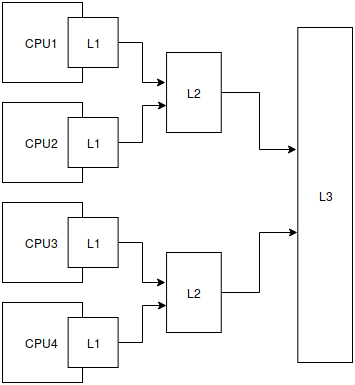
\includegraphics[width=0.3\textwidth]{images/Diagram_1.png}
		\caption[]{Schematic representation of the Neumann model}
	\end{center}	
\end{figure}

\section{Use case}

\section{Usage of Internet of Things}

\section{The research question}

\section{The envisioned architecture}

\section{Weekly milestones}


a use case – a short story to illustrate the why & how
a description of how and why IoT/P2P will be used
a couple of hypotheses, i.e., "good questions" that do not have obvious answers, and that you seek to answer in your project
a sketch of the envisioned architecture
some rough and realistic weekly milestones



\bibliography{ref}
\bibliographystyle{ieeetr}

\end{document}
